\documentclass[xcolor=table]{beamer}
\usepackage{graphicx}
\usetheme{Berlin}
\usecolortheme{beaver}
\useoutertheme{infolines}
\title{ANN \& R Programming}
\date {~}
\author{Jaishankar Hebballi(13030142017)}
\setbeamertemplate{items}[ball]
%\logo{\scalebox{0.1}{\includegraphics{openssh.jpg}}}
\begin{document}
\maketitle{}
\AtBeginSection[]
{
\begin{frame}[shrink]{Overview}
\tableofcontents[currentsection, hideothersubsections]

\end{frame}
}
\section{Character Recognition}
\begin{frame}
\textbf {Character Recognition} \\
Many Optical Character recognition softwares (OCR) exist. 
Their basic functionality is to be able to parse and guess the characters that may be handwritten or typed.
But my scope is not as big. In this project a very basic character recognition is implemented. Two learning rules are implemented
to guess the correct output. Two kinds of recognition is done in this project.
\begin{itemize} [<+->]
\item Pattern Classification	
\item Pattern Association
\end{itemize}

\end{frame}

\section{Packages Used}
\begin{frame}[fragile]

\begin{itemize} [<+->]
\item \verb+RSNNS+
\item \verb+pixmap+
\item \verb+gWidgets+
\item \verb+gWidgets2+
\item \verb+gWidgetsRGtk+ 
\item \verb+gWidgets2RGtk2+
\item \verb+stringr+
\item \verb+cairo+
\end{itemize}
All these packages can be installed from the repository using \verb+install.packages(package_name)+
\end{frame}

\section{My Goal}
\begin{frame}
\textbf {My Goal} \\

Very Basic Pattern Recognition\\

\begin{itemize} [<+->]
\item Accept images from the user
\item Train the network with a few known input images.
\item Make the Network guess the unkown input.

\end{itemize}
\end{frame}

\section{Input}
\begin{frame}[fragile]
\textbf {Encode Input} \\
\begin{itemize} [<+->]
\item From the user get an image of 9*9 pixels.
\item The Image can contain any alphabet in Capital letters
\item Transform the input into a matrix of bi-polar numbers which will be fed into the network. 
\end{itemize}
\end{frame}

\section{Output}
\begin{frame}[fragile]
\textbf {Decode Output} \\
Pattern Classification
\begin{itemize} [<+->]
\item The network will output a sequence of binary numbers
\item Decode this number into an ASCII character
\item Display the correct character to the user
\end{itemize}
Pattern Association
\begin{itemize} [<+->]
\item The network will output a sequence of binary numbers
\item Decode this number into an pixmap image
\item Plot or draw this image on the window
\end{itemize}
\end{frame}

\section{Learning Rules}
\begin{frame}
\textbf{Learning Rules}\\
\begin{itemize}
 \item Hebbian Learning Rule
 \item Perceptron Rule
 \item Delta Learning Rule
 \item Backpropagation 
\end{itemize}
\end{frame}

\section{Error Plots}
\begin{frame}
\textbf{Error Graphs}
Mean Error against epoch times. The graphs tell us how the learning has taken place. 
\begin{itemize}
 \item MLP Backpropagation (classification)
 \item My Perceptron Implementation
 \item Delta Learning
 \item MLP Backpropagation (association)
\end{itemize}
\end{frame}

\begin{frame}
 My Perceptron Error Reduction Curve\\
 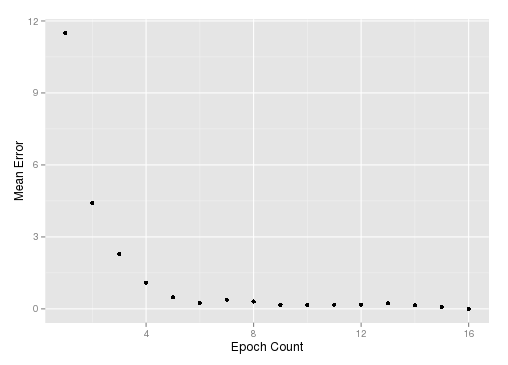
\includegraphics[scale=0.4]{myPerceptronError.png}
 
\end{frame}

\begin{frame}
 
 Delta Rule Error Reduction Curve\\
 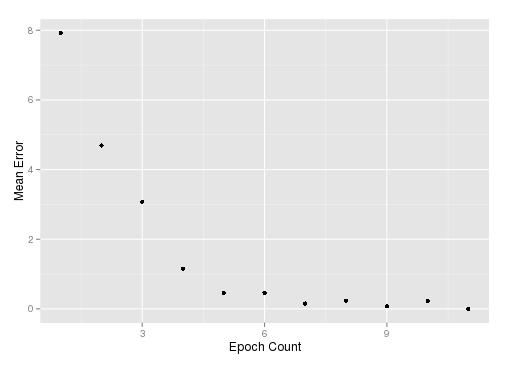
\includegraphics[scale=0.4]{deltaError.png}
 
\end{frame}
\begin{frame}
 Multi-Layer Perceptron (Classification) Error Reduction Curve\\
 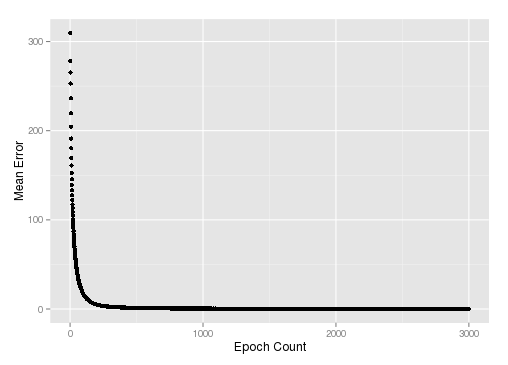
\includegraphics[scale=0.4]{mlpClassification.png}
 RSNNS Package network
\end{frame}
\begin{frame}
 Multi-Layer Perceptron (Association) Error Reduction Curve\\
 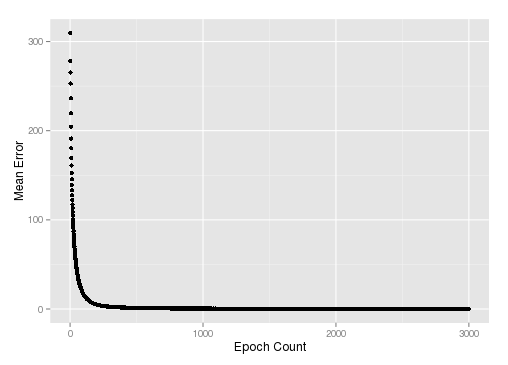
\includegraphics[scale=0.4]{mplAssociation.png}
 RSNNS Package network
\end{frame}
\begin{frame}
 Comparison between all Four\\
 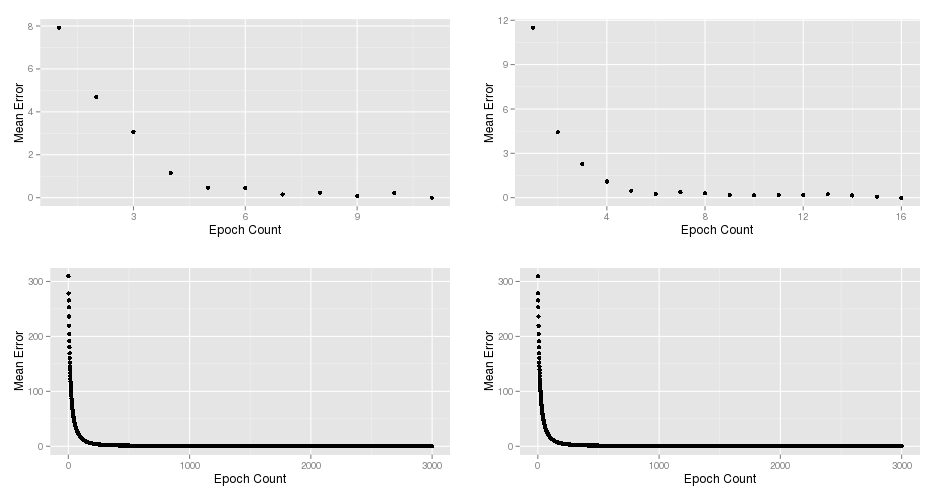
\includegraphics[scale=0.35]{all.png}
 
\end{frame}

\section{Performance Times}
\begin{frame}
\textbf{Performance Times}
\begin{itemize}
 \item MLP Backpropagation (classification) (6.650 sec)
 \item My Perceptron Implementation (3.155 sec)
 \item Delta Learning (2.817 sec)
 \item Hebbian Rule (association) (0.023 sec)
 \item MLP Backpropagation (association) (8.685 sec)
\end{itemize}

\end{frame}


\section{References}
\begin{frame}{References}
\begin{thebibliography}{widest entry}
\bibitem{cite_key1} \url{Fundamentals of Neural Networks (Laurene Fausett)}
\bibitem{cite_key2} {Neural Networks in R Using the Stuttgart Neural Network Simulator: RSNNS}
\bibitem{cite_key3} {Packages manual pages}
\bibitem{cite_key4} \url{Introduction to Neural Networks using MATLAB}
\end{thebibliography}

\end{frame}

\begin{frame}{Thank you}
\begin{center}
\vskip1cm
Thank You!
\end{center}
\end{frame}

\end{document}
